\documentclass{bmvc2k}

%% Enter your paper number here for the review copy
%\bmvcreviewcopy{??}  % Uncomment for review submission with line numbers

\title{Unsupervised Panoptic Segmentation via\\Depth-Semantic Pseudo-Label Compositing}

% Anonymized for review
\addauthor{Anonymous}{anonymous@email.com}{1}
\addinstitution{Anonymous Institution}

\runninghead{Anonymous}{Depth-Semantic Pseudo-Label Compositing}

% Macros
\def\eg{\emph{e.g}\bmvaOneDot}
\def\Eg{\emph{E.g}\bmvaOneDot}
\def\etal{\emph{et al}\bmvaOneDot}
\def\ie{\emph{i.e}\bmvaOneDot}

\usepackage{amsmath}
\usepackage{amssymb}
\usepackage{booktabs}
\usepackage{multirow}
\usepackage{xcolor}
\usepackage{xspace}
\usepackage{placeins}  % for \FloatBarrier

% Custom commands
\newcommand{\method}{Ours\xspace}
\newcommand{\pqt}{PQ\textsubscript{th}\xspace}
\newcommand{\pqs}{PQ\textsubscript{st}\xspace}

%-------------------------------------------------------------------------
\begin{document}

\maketitle

\begin{abstract}
Unsupervised panoptic segmentation seeks to partition images into semantic regions and object instances without any manual annotation---a task that demands both categorical understanding and individual object separation from unlabeled data alone.
%
The only existing method for scene-centric unsupervised panoptic segmentation, CUPS~\cite{hahn2025cups}, relies on stereo video sequences and optical flow to generate pseudo-labels, coupling its applicability to multi-view geometry that is unavailable in standard monocular imagery.
%
We observe that these two requirements---semantic grouping and instance separation---can be decomposed into complementary signals from frozen foundation models: a feature-clustering model encodes appearance and texture sufficient for semantic categories, while a monocular depth estimator encodes geometric structure sufficient for object boundaries.
%
Building on this decomposition, we compose CAUSE-TR overclustered features for semantics and Depth Anything~3 gradient thresholding for instances into panoptic pseudo-labels, then train a Cascade Mask R-CNN with a frozen DINOv3 ViT-B/16 backbone and EMA-guided self-training---all from single RGB images, with no stereo pairs, no video, and no optical flow.
%
On Cityscapes under the standard 27-class evaluation protocol, our method achieves \textbf{32.76\% PQ}, surpassing CUPS by \textbf{+5.0 PQ} and improving thing-class quality from 17.7\% to \textbf{34.1\% \pqt}---a +16.4 point gain using strictly less input data.
\end{abstract}

\begin{figure*}[t]
\centering
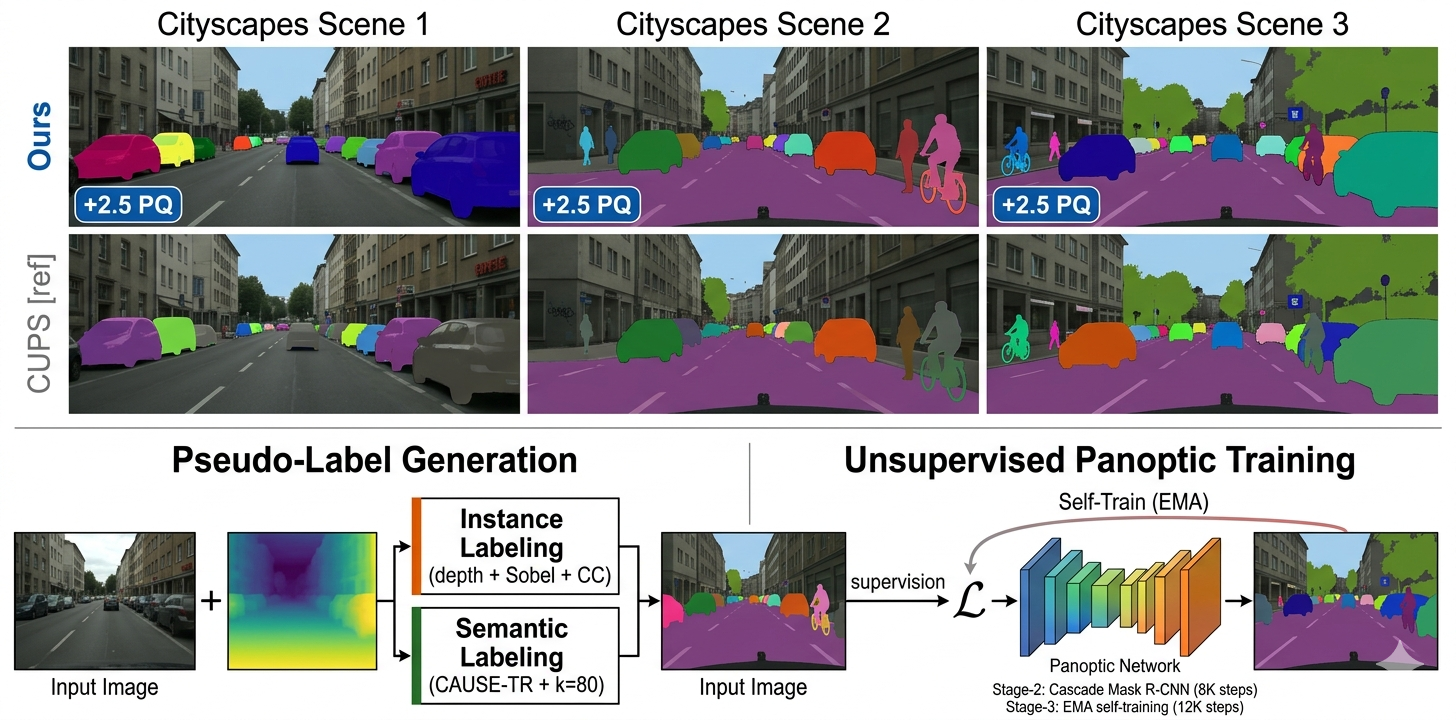
\includegraphics[width=\textwidth]{figures/fig1_overview_ai.png}
\caption{\textbf{Overview and results.} Top: panoptic predictions (ours, Stage-3) vs CUPS pseudo-labels on three Cityscapes validation scenes. Bottom left: pseudo-label generation using monocular depth (DAv3) for instance labeling and CAUSE-TR overclustering for semantic labeling. Bottom right: panoptic network trained on pseudo-labels with EMA self-training. Our method achieves PQ=32.76\%, surpassing CUPS (27.8\%) by +5.0 PQ using only monocular images.}
\label{fig:overview}
\end{figure*}

%-------------------------------------------------------------------------
\section{Introduction}
\label{sec:intro}

Panoptic segmentation unifies semantic segmentation (assigning each pixel a class label) with instance segmentation (distinguishing individual objects), producing a complete scene understanding where every pixel belongs to either a countable ``thing'' instance or an amorphous ``stuff'' region~\cite{kirillov2019panoptic}. Supervised panoptic models have achieved remarkable accuracy, but their dependence on dense per-pixel annotations---which cost approximately 1.5 hours per image on Cityscapes~\cite{cordts2016cityscapes}---severely limits scalability to new domains and categories.

Unsupervised panoptic segmentation removes this bottleneck by training on pseudo-labels derived entirely from pretrained models, requiring no human annotation whatsoever. The core challenge is that semantic and instance cues must be recovered independently and then composed into a coherent panoptic representation. Prior work has approached this through two main directions: unsupervised semantic segmentation methods such as PiCIE~\cite{cho2021picie}, STEGO~\cite{hamilton2022stego}, and CAUSE~\cite{kim2025cause} recover pixel-level class assignments from self-supervised features but do not separate individual object instances; unsupervised instance segmentation methods such as CutLER~\cite{wang2023cutler} and FreeSOLO~\cite{wang2022freesolo} detect objects without labels but lack semantic class understanding. The only existing method that addresses the full panoptic task without supervision is CUPS~\cite{hahn2025cups}, which achieves PQ=27.8\% on Cityscapes by leveraging stereo video and optical flow for pseudo-label generation---geometric signals that are unavailable in typical monocular deployment scenarios.

We observe that the complementary structure of the panoptic task admits a natural decomposition: semantic pseudo-labels can be generated from frozen feature-clustering models that encode appearance and texture, while instance pseudo-labels can be derived from monocular depth estimators that encode geometric structure. Neither signal alone suffices---semantic features cannot distinguish adjacent objects of the same class, and depth maps cannot assign semantic categories---but their composition produces panoptic pseudo-labels of sufficient quality to train a strong segmentation network.

Building on this observation, we propose a two-phase pipeline (Figure~\ref{fig:overview}). In Phase~1, we generate panoptic pseudo-labels by composing two frozen foundation models: (i)~DINOv2~\cite{oquab2024dinov2} with a CAUSE-TR~\cite{kim2025cause} projection head for semantic features, overclustered with $k{=}80$ K-means centroids; and (ii)~Depth Anything~3~\cite{lin2025da3} for monocular depth, from which instance boundaries are extracted via Sobel gradient thresholding. A depth-split-ratio classifier (Eq.~\ref{eq:splitratio}) separates thing from stuff classes without ground-truth labels. In Phase~2, we train a Cascade Mask R-CNN~\cite{cai2021cascade} with a frozen DINOv3~\cite{fang2025dinov3} backbone on these pseudo-labels, following the CUPS training protocol with DropLoss and CopyPaste augmentation, then apply EMA-guided self-training for 8,000 steps.

Our contributions are:
\begin{itemize}
\item \textbf{A monocular pseudo-label generation pipeline} that composes frozen semantic clustering (CAUSE-TR, $k{=}80$) and monocular depth estimation (DAv3) to produce panoptic pseudo-labels achieving PQ=27.37\% without any manual annotation or multi-view geometry---exceeding the quality of CUPS pseudo-labels (PQ=26.5\%) that require stereo video and optical flow.

\item \textbf{A systematic depth model estimation} showing that pseudo-label quality scales monotonically with depth estimator accuracy (SPIdepth: 19.41 \pqt, DAv2: 20.20, DAv3: 20.90), while alternative splitting algorithms (Canny, watershed, multiscale Sobel) provide no improvement---establishing depth quality, not post-processing, as the binding constraint.

\item \textbf{State-of-the-art unsupervised panoptic segmentation} on Cityscapes, achieving PQ=32.76\% with DINOv3 ViT-B/16 + Cascade Mask R-CNN + EMA self-training, surpassing CUPS (27.8\%) by +5.0 PQ and improving \pqt from 17.7\% to 34.1\% (+16.4 points).

\item \textbf{An analysis of self-training scaling behavior} demonstrating that EMA self-training gains scale with teacher quality: +1.25 PQ for ResNet-50 (24.68\% to 25.93\%) versus +4.89 PQ for DINOv3 (27.87\% to 32.76\%), with thing-class quality as the primary beneficiary (+10.9 \pqt for DINOv3).
\end{itemize}

%-------------------------------------------------------------------------
\section{Related Work}
\label{sec:related}

\noindent\textbf{Unsupervised semantic segmentation.}
Clustering dense features from self-supervised vision transformers has emerged as the dominant paradigm. PiCIE~\cite{cho2021picie} introduced pixel-level invariance and equivariance constraints for clustering. STEGO~\cite{hamilton2022stego} improved upon this by distilling feature correspondences from DINO~\cite{caron2021dino} into a contrastive segmentation head. HP~\cite{seong2023hp} and EAGLE~\cite{kim2024eagle} further refined clustering quality through leveraging hidden positives and entropy-guided learning, respectively. CAUSE~\cite{kim2025cause} introduced a causal framework with a modularity codebook that trains a Segment\_TR projection head, producing 90-dimensional features better suited for clustering than raw backbone features. Our work builds directly on CAUSE-TR features but addresses a critical failure mode: at the standard $k{=}27$ cluster count, 14 of 27 centroids are dead and seven evaluation classes receive zero IoU. We resolve this through overclustering with $k{=}80$ centroids.

\noindent\textbf{Unsupervised instance segmentation.}
Without per-object annotations, instance segmentation must rely on appearance or geometric cues. FreeSOLO~\cite{wang2022freesolo} generates coarse masks from self-supervised features and trains a SOLO detector. CutLER~\cite{wang2023cutler} extends this with MaskCut---iterative normalized cuts on DINO self-attention maps. CuVLER~\cite{arica2024cuvler} extends CutLER with DINOv2 features for improved mask quality. DINOSAUR~\cite{seitzer2023dinosaur} applies slot attention to DINO features for object-centric decomposition. U2Seg~\cite{niu2024u2seg} combines CutLER-style instance proposals with STEGO semantic masks into a unified unsupervised panoptic framework. However, all these methods operate on appearance features alone and struggle with adjacent same-class objects. Our depth-guided splitting approach is complementary: it exploits the geometric prior that physically distinct objects at different depths produce gradient discontinuities.

\noindent\textbf{Monocular depth estimation.}
Self-supervised depth estimation has matured rapidly. Monodepth2~\cite{godard2019monodepth2} established the photometric self-supervision framework, and SPIdepth~\cite{lavreniuk2025spidepth} achieves state-of-the-art self-supervised results. In parallel, foundation-model-scale supervised depth estimators---Depth Anything~\cite{yang2024da1}, Depth Anything~V2~\cite{yang2024da2}, and Depth Anything~3~\cite{lin2025da3}---have demonstrated that training on massive synthetic datasets produces depth maps of unprecedented quality. We leverage these depth maps as an instance boundary signal: Sobel gradient thresholding on depth maps produces a binary edge mask that, combined with per-class connected component analysis, yields instance pseudo-labels.

\noindent\textbf{Unsupervised panoptic segmentation.}
CUPS~\cite{hahn2025cups} is, to our knowledge, the only prior method that directly addresses unsupervised panoptic segmentation on scene-centric imagery. CUPS generates instance pseudo-labels through SF2SE3 motion segmentation from scene flow extracted from stereo video, and semantic pseudo-labels through a DINO-based semantic network with depth-guided inference. CUPS achieves PQ=27.8\% on Cityscapes, advancing the state of the art by 9.4 PQ over the previous best. Our method adopts the CUPS training protocol (Stage-2 + Stage-3) but replaces the pseudo-label generation pipeline entirely: where CUPS requires stereo pairs, video sequences, and optical flow, we use only monocular images with frozen foundation models. This simplification does not sacrifice quality---our pseudo-labels achieve comparable \pqt (20.90 vs 17.7) and our trained network surpasses CUPS by +5.0 PQ---while substantially reducing the data requirements for deployment.

\noindent\textbf{Vision foundation models.}
Our pipeline leverages frozen features from DINOv2~\cite{oquab2024dinov2} for semantic clustering and DINOv3~\cite{fang2025dinov3} as the downstream network backbone. DINOv3 scales self-supervised pretraining to 1.7B images with improved dense feature quality, offering models from ViT-S to ViT-g; we use the ViT-B/16 variant ($\sim$86M parameters). At the detection level, Mask2Former~\cite{cheng2022mask2former} provides a universal architecture for panoptic, instance, and semantic segmentation that serves as the supervised upper bound.

%-------------------------------------------------------------------------
\section{Method}
\label{sec:method}

\subsection{Overview}

Our pipeline proceeds in two sequential phases. In Phase~1, we generate per-image panoptic pseudo-labels by independently estimating pixel-level semantic assignments from a frozen feature-clustering model and instance assignments from a monocular depth estimator, then merging the two modalities into a coherent panoptic representation. In Phase~2, we train a Cascade Mask R-CNN~\cite{cai2021cascade} on these pseudo-labels following the CUPS training protocol~\cite{hahn2025cups}, and apply EMA-guided self-training to iteratively refine predictions. The pseudo-label generator is entirely absent at inference time: the deployed network sees only a single RGB image.

\begin{figure*}[t]
\centering
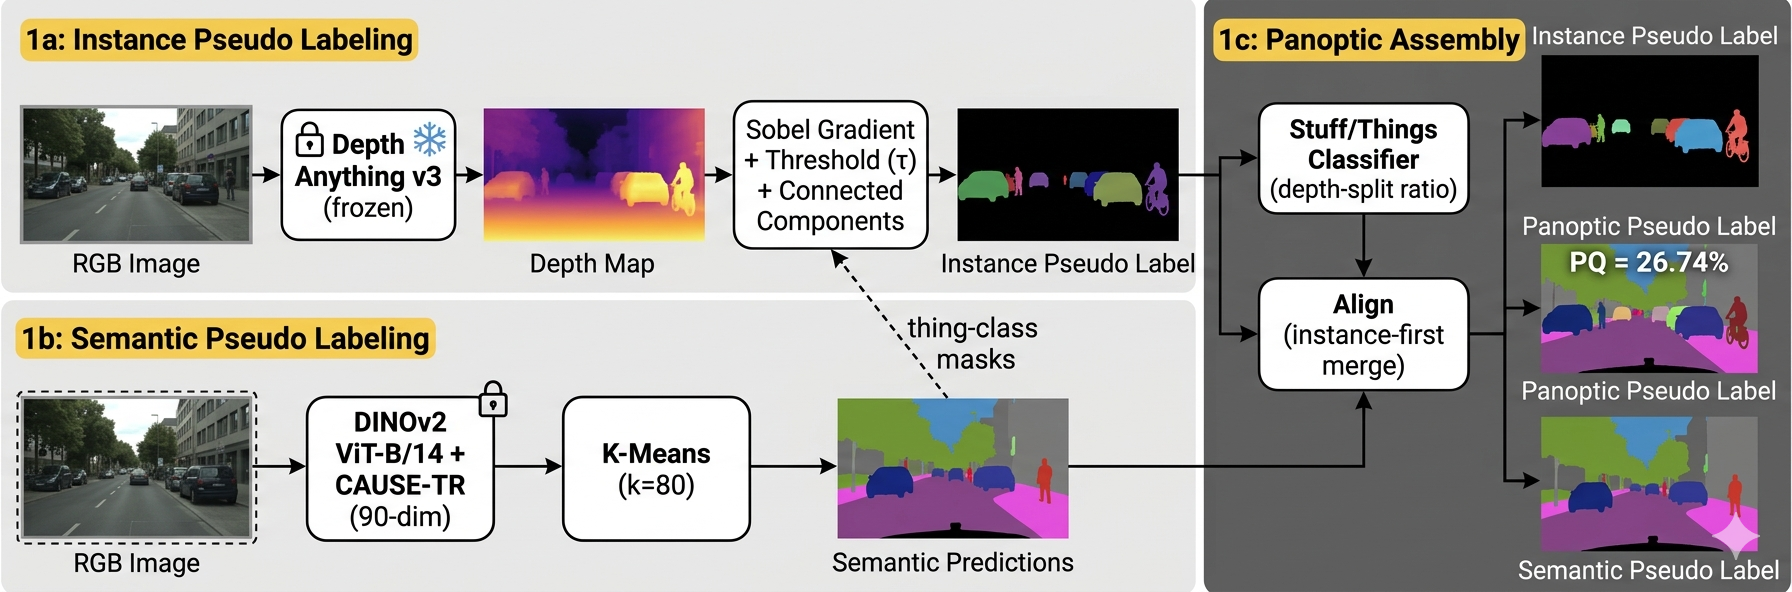
\includegraphics[width=\textwidth]{figures/fig2_pl_pipeline_ai.png}
\caption{\textbf{Stage~1: Pseudo-label generation.} 1a~(top): Instance pseudo labeling---Sobel gradient thresholding on monocular depth (DAv3) splits thing-class regions into individual instances via connected components. 1b~(bottom): Semantic pseudo labeling---CAUSE-TR features clustered with $k{=}80$ K-means overclustering. 1c~(right): Panoptic assembly aligns the two signals using instance-first merging with a depth-split-ratio stuff/things classifier.}
\label{fig:pl_pipeline}
\end{figure*}

\subsection{Semantic Pseudo-Label Generation}
\label{sec:semantic}

The central challenge in generating semantic pseudo-labels without supervision is recovering the full set of target classes from a pretrained feature space. The CAUSE~\cite{kim2025cause} framework addresses this by training a cluster probe---a set of 27 centroids matched one-to-one to semantic classes---on top of its Segment\_TR feature head. However, a confusion matrix analysis across all 500 Cityscapes validation images reveals that 14 of the 27 learned centroids are dead: they never win the argmax competition for any pixel. As a result, seven of the 19 evaluation classes---fence, pole, traffic light, traffic sign, rider, train, and motorcycle---receive exactly zero IoU. The failure follows systematic absorption patterns: fence pixels are classified as wall (70\%) and building (13\%), pole pixels as building (65\%) and vegetation (10\%).

The 90-dimensional Segment\_TR features are essential---clustering raw 768-dimensional DINOv2~\cite{oquab2024dinov2} tokens directly achieves only 46.0\% mIoU versus 61.3\% for Segment\_TR features at $k{=}300$, a gap of 15.3 points. We address the centroid collapse problem by \emph{overclustering}: fitting $k{=}80$ centroids on L2-normalized features, with each centroid mapped to one of 19 Cityscapes classes via majority vote. This many-to-one mapping allows rare categories to claim dedicated cluster regions. We select $k{=}80$ as the smallest value at which all seven collapsed classes reliably attract at least one dedicated centroid. CUPS~\cite{hahn2025cups} reports a similar benefit from overclustering (their Table~7b), but applies it to their own jointly-trained semantic network---a different feature space. Our contribution is the diagnosis of centroid collapse in frozen CAUSE-TR features and the empirical finding that $k{=}80$ is the minimum threshold for full class recovery.

\begin{figure}[t]
\centering
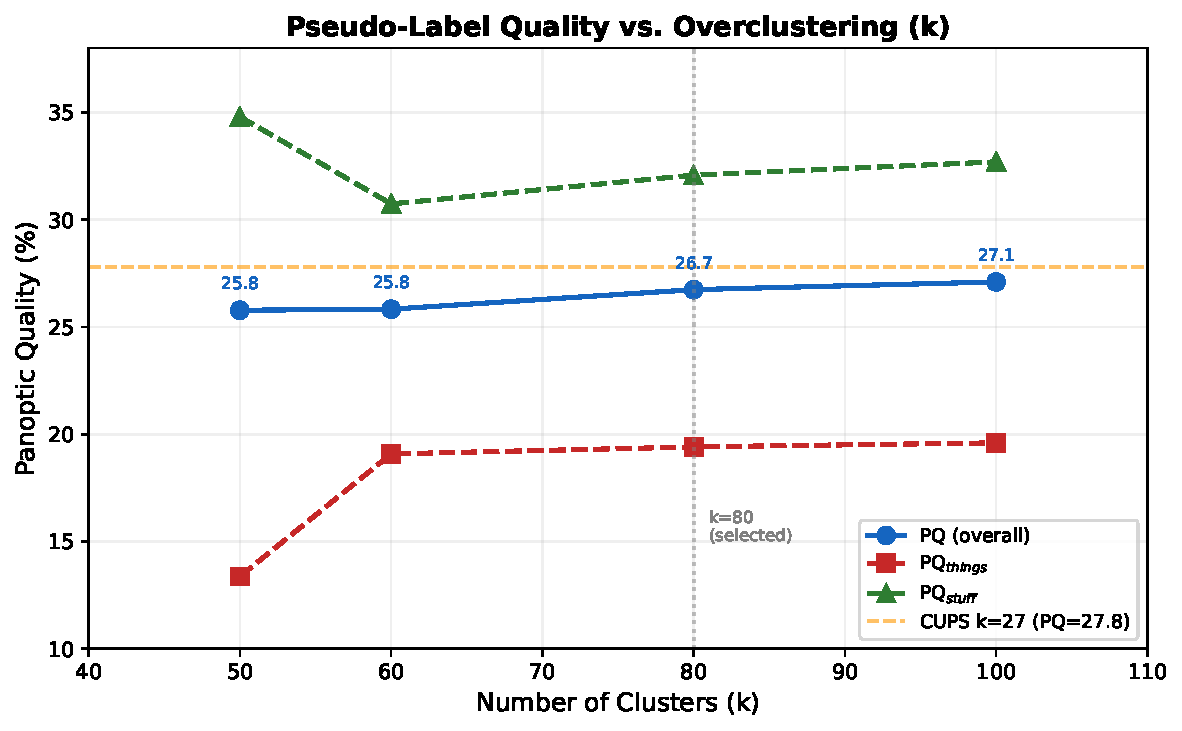
\includegraphics[width=0.55\columnwidth]{figures/fig4_ksweep.pdf}
\caption{\textbf{Pseudo-label quality vs.\ overclustering count $k$.} PQ increases monotonically from 25.78\% ($k{=}50$) to 27.10\% ($k{=}100$). \pqt jumps sharply between $k{=}50$ and $k{=}60$ as collapsed classes recover. We select $k{=}80$ as the operating point.}
\label{fig:ksweep}
\end{figure}

Feature extraction applies a 322$\times$322 sliding window (stride 161) with horizontal flip over the frozen Segment\_TR head, followed by L2-normalization. This ensures k-means equivalence to cosine similarity:
\begin{equation}
\|\mathbf{f} - \mathbf{c}\|^2 = \|\mathbf{f}\|^2 + \|\mathbf{c}\|^2 - 2\mathbf{f}^\top\mathbf{c} = 2(1 - \mathbf{f}^\top\mathbf{c})
\label{eq:cosine}
\end{equation}
The raw cluster assignments (integers 0--79) are saved directly as pseudo-labels, preserving full granularity. Class correspondence is resolved at evaluation time via Hungarian matching, identical to the CUPS protocol.

\subsection{Depth-Guided Instance Pseudo-Label Generation}
\label{sec:instance}

Depth encodes a prior that naturally resolves instance ambiguity in driving scenes: physically distinct objects at different distances produce discontinuities in the depth map. Given an image, we estimate a dense depth map using Depth Anything~3 (DAv3)~\cite{lin2025da3}. The depth map is smoothed with a Gaussian filter ($\sigma{=}1.0$), and the gradient magnitude is computed via a Sobel filter:
\begin{equation}
G(p) = \sqrt{G_x(p)^2 + G_y(p)^2}, \quad G_x = \frac{\partial d_\sigma}{\partial x},\; G_y = \frac{\partial d_\sigma}{\partial y}
\label{eq:sobel}
\end{equation}
A binary depth edge mask is obtained by thresholding:
\begin{equation}
\mathcal{E}_\text{depth} = \{p : G(p) > \tau\}
\label{eq:edges}
\end{equation}

For each thing class $k$, we compute the split mask $S_k = M_k \cap \neg\mathcal{E}_\text{depth}$ and run connected component analysis on $S_k$. Components smaller than $A_\text{min}$ pixels are discarded, and a three-pixel dilation step reclaims boundary pixels. We set $\tau{=}0.03$ and $A_\text{min}{=}1000$ based on the depth model ablation in Section~\ref{sec:depth_ablation}.

A limitation that this approach cannot overcome is the \emph{co-planarity failure mode}: when multiple instances occupy the same depth plane (e.g.,~pedestrians standing side by side), the depth map shows no gradient at their shared boundary.

\subsection{Panoptic Pseudo-Label Assembly}
\label{sec:assembly}

Separating thing from stuff classes without ground-truth labels requires a novel classifier. For class $k$ with binary mask $M_k$, we define the \emph{depth-split ratio}:
\begin{equation}
R_\text{split}(k) = \frac{\mathbb{E}_I[\text{CC}(M_k \cap \neg\mathcal{E}_\text{depth})]}{\mathbb{E}_I[\text{CC}(M_k)]}
\label{eq:splitratio}
\end{equation}
where $\text{CC}(\cdot)$ counts connected components and $\mathbb{E}_I[\cdot]$ averages over training images. Thing classes have $R_\text{split} \gg 1$ because depth edges split adjacent objects; stuff classes have $R_\text{split} \approx 1$. The top 8 classes by $R_\text{split}$ are assigned as things, after excluding large-coverage classes with artificially high ratios.

We assemble panoptic pseudo-labels using an instance-first merging strategy: instance masks are placed in descending order of area, each receiving a semantic class by majority vote. Stuff segments fill remaining pixels. The resulting pseudo-labels achieve PQ=27.37\% with DAv3 instances---exceeding CUPS pseudo-labels (PQ=26.5\%) that require stereo video and optical flow.

\begin{figure*}[t]
\centering
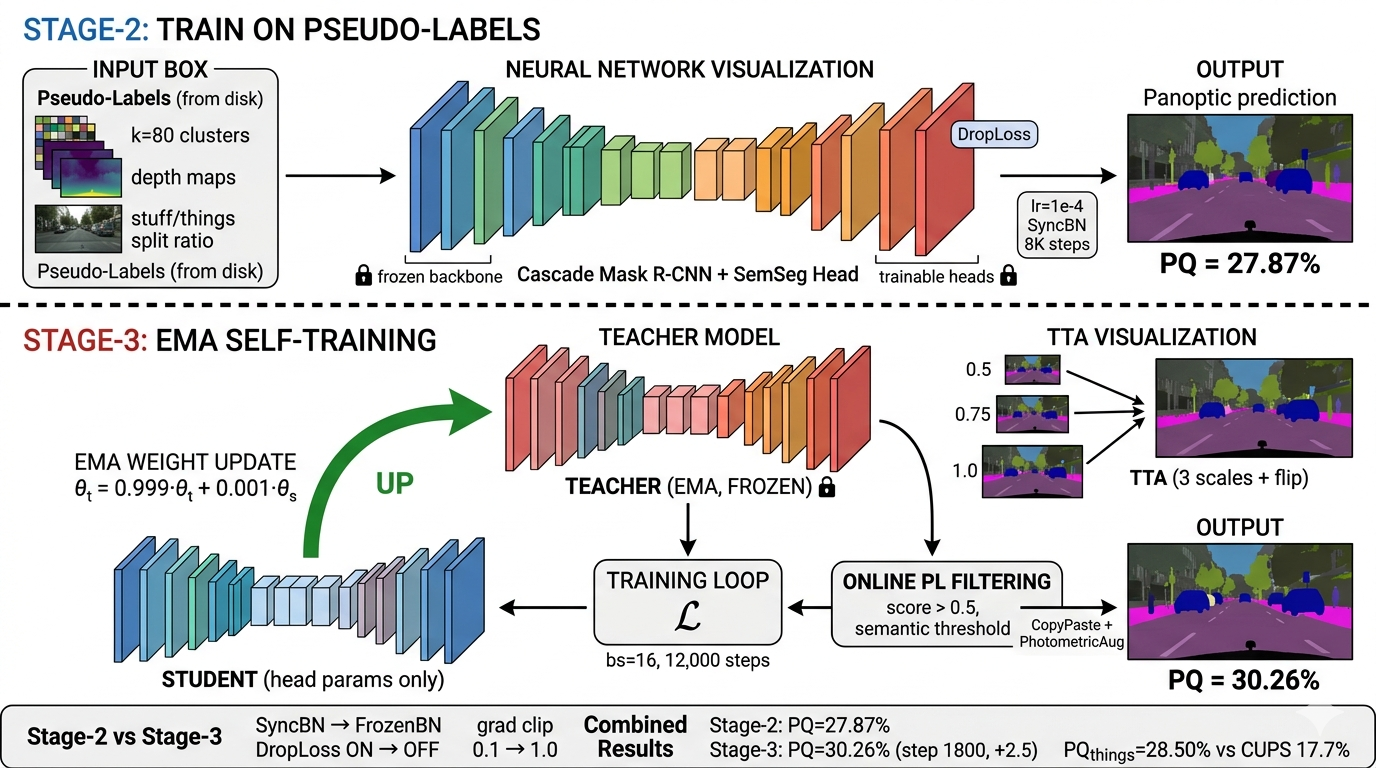
\includegraphics[width=\textwidth]{figures/fig3_training_ai.png}
\caption{\textbf{Network training pipeline.} Stage-2~(top): Cascade Mask R-CNN with frozen DINOv3 ViT-B/16 backbone trained on pseudo-labels from disk with DropLoss, producing PQ=27.87\%. Stage-3~(bottom): EMA teacher generates online pseudo-labels via TTA (3~scales + flip); student trains on confidence-filtered predictions; EMA update ($\alpha{=}0.999$) closes the self-training loop over 8,000 steps, achieving PQ=32.76\%.}
\label{fig:training}
\end{figure*}

\subsection{Network Training}
\label{sec:training}

We adopt the two-stage protocol from CUPS~\cite{hahn2025cups}. In Stage~2, a Cascade Mask R-CNN with a frozen DINOv3 ViT-B/16~\cite{fang2025dinov3} backbone (\texttt{facebook/dinov3-vitb16-pretrain-lvd1689m}) is trained on the $k{=}80$ pseudo-labels. The recipe includes DropLoss, which assigns per-proposal loss weights:
\begin{equation}
w_i = 1 - \mathbb{1}[\max_j \text{IoU}(b_i, g_j) \leq \tau_\text{drop}]
\label{eq:droploss}
\end{equation}
where $\tau_\text{drop}{=}0.4$. Predictions with low IoU to any pseudo-label receive zero weight, preventing penalization of correct detections absent from noisy pseudo-labels. The recipe also includes CopyPaste augmentation, resolution jitter (384--512px), gradient clipping (norm 0.1), and label smoothing ($\epsilon{=}0.1$). These components are credited in full to CUPS.

In Stage~3, a teacher network is initialized as a copy of Stage~2 and updated via EMA~\cite{tarvainen2017mean}:
\begin{equation}
\boldsymbol{\theta}_T^{(t+1)} = \alpha \cdot \boldsymbol{\theta}_T^{(t)} + (1 - \alpha) \cdot \boldsymbol{\theta}_S^{(t)}
\label{eq:ema}
\end{equation}
where $\alpha{=}0.999$. The teacher generates predictions using TTA at three scales (0.5$\times$, 0.75$\times$, 1.0$\times$) with horizontal flip. The student is retrained on the teacher's high-confidence outputs for 8,000 steps with gradient clipping at norm 1.0, frozen BatchNorm, and DropLoss disabled. This self-training paradigm follows Noisy Student~\cite{xie2020noisy} principles, where a stronger teacher iteratively generates pseudo-labels consumed by the student.

%-------------------------------------------------------------------------
\section{Experiments}
\label{sec:experiments}

\subsection{Experimental Setup}

\paragraph{Dataset and evaluation protocol.}
We evaluate on the Cityscapes~\cite{cordts2016cityscapes} validation set (500 images, 1024$\times$2048). All results use the 27-class CAUSE+Hungarian evaluation protocol from CUPS~\cite{hahn2025cups}: $k{=}80$ predicted clusters are matched to 27 Cityscapes categories via the Hungarian algorithm, and panoptic quality (PQ)~\cite{kirillov2019panoptic} is decomposed into stuff (\pqs) and thing (\pqt) components. This protocol ensures a direct, apples-to-apples comparison with CUPS.

\paragraph{Training details.}
Stage-2 trains a Cascade Mask R-CNN~\cite{cai2021cascade} with a frozen DINOv3 ViT-B/16~\cite{fang2025dinov3} backbone on our pseudo-labels for 8{,}000 steps, following the CUPS training recipe (DropLoss~\cite{hahn2025cups}, CopyPaste augmentation~\cite{ghiasi2021copypaste}, learning rate $1{\times}10^{-4}$ with linear warmup). Stage-3 applies EMA-guided self-training for an additional 8{,}000 steps with confidence thresholding. All training uses two GTX~1080~Ti GPUs (11\,GB each) with PyTorch~2.1.2 and Detectron2~0.6, seed 42. For cross-dataset generalization, we additionally evaluate on MOTS, KITTI, Mapillary Vistas~v2~\cite{neuhold2017mapillary}, and COCO-Stuff-27 without any fine-tuning.

\paragraph{Notation.}
Throughout this section, ``CC-only'' denotes connected-component instance labeling without depth-guided splitting; $\tau$ denotes the Sobel gradient threshold used for depth edge detection; and $A_\text{min}$ is the minimum component area filter. We report PQ, \pqt, and \pqs averaged over the 27-class protocol unless otherwise noted.

\subsection{Comparison with State of the Art}

Table~\ref{tab:sota} compares our method against all published unsupervised panoptic segmentation methods on Cityscapes.

\begin{table}[t]
\centering
\caption{Comparison with state-of-the-art unsupervised panoptic segmentation on Cityscapes val. $^\dagger$~denotes methods requiring stereo video or optical flow. Numbers for DepthG+CutLER and U2Seg are from~\cite{hahn2025cups}.}
\label{tab:sota}
\small
\begin{tabular}{@{}lccccc@{}}
\toprule
Method & Data & PQ & \pqt & \pqs & SQ \\
\midrule
DepthG + CutLER & CS+IN & 16.1 & 3.0 & 25.7 & 45.4 \\
U2Seg~\cite{niu2024u2seg} & COCO+IN & 18.4 & 10.2 & 24.3 & 55.8 \\
CUPS$^\dagger$~\cite{hahn2025cups} & CS (stereo) & 27.8 & 17.7 & 35.1 & 57.4 \\
\midrule
\textbf{Ours -- Stage~2} & CS (mono) & 27.87 & 23.2 & 30.6 & 57.8 \\
\textbf{Ours -- Stage~3} & CS (mono) & \textbf{32.76} & \textbf{34.1} & 32.0 & \textbf{62.6} \\
\bottomrule
\end{tabular}
\end{table}

Three observations emerge. First, Stage-2 alone---before any self-training---already matches CUPS in overall PQ (27.87 vs.\ 27.8) despite using strictly monocular input, while improving \pqt from 17.7\% to 23.2\% (+5.5 points). Second, Stage-3 self-training amplifies this advantage to \textbf{+5.0 PQ} overall and \textbf{+16.4 \pqt} (17.7\% $\to$ 34.1\%), the largest thing-class improvement reported on this benchmark. Third, our \pqs (32.0\%) falls $-$3.1 points below CUPS (35.1\%); a per-class analysis (Appendix~C) attributes this entirely to 7 non-standard CAUSE classes on which our model achieves PQ$<$1\%, because the frozen CAUSE-TR clustering cannot recover classes that receive zero centroids---whereas CUPS learns these classes end-to-end. On the remaining 16 well-represented classes, our average PQ is 49.0\%.

\paragraph{Pretraining caveat.}
While our method requires only monocular input at deployment, DAv3 was itself pretrained with multi-view geometry. The ``monocular'' characterization refers to inference-time data requirements, not foundation model pretraining.

\subsection{Ablation Studies}
\label{sec:ablations}

We structure our ablations as a progressive investigation. Each sub-experiment isolates one factor while holding all others fixed.

\begin{table*}[t]
\centering
\caption{Ablation studies on Cityscapes val. (a)~Pseudo-label quality before network training. (b)~Instance quality: depth model (top) and splitting algorithm (bottom, DAv3 fixed). (c)~Backbone effect (Stage-2). (d)~Self-training scaling.}
\label{tab:ablations}
\small
\begin{tabular}{@{}c@{\hspace{18pt}}c@{}}
% ---- Left column ----
\begin{minipage}[t]{0.46\textwidth}
\centering
\textbf{(a) Pseudo-Label Quality} \\[4pt]
\begin{tabular}{@{}lccc@{}}
\toprule
Source & PQ & \pqt & \pqs \\
\midrule
CUPS Stage-1~\cite{hahn2025cups} & 26.5 & 17.7 & --- \\
Ours -- CC-only & 23.1 & 14.9 & 28.2 \\
Ours -- SPIdepth & 26.74 & 19.41 & 32.08 \\
Ours -- DAv3 & \textbf{27.37} & \textbf{20.90} & 32.08 \\
\bottomrule
\end{tabular}
\\[12pt]
\textbf{(c) Backbone Ablation (Stage-2)} \\[4pt]
\begin{tabular}{@{}lccc@{}}
\toprule
Backbone & PQ & \pqt & \pqs \\
\midrule
DINOv2 ResNet-50 & 24.68 & 19.1 & 28.0 \\
DINOv3 ViT-B/16 & \textbf{27.87} & \textbf{23.2} & \textbf{30.6} \\
\bottomrule
\end{tabular}
\end{minipage}
&
% ---- Right column ----
\begin{minipage}[t]{0.46\textwidth}
\centering
\textbf{(b) Instance Quality: Depth Model vs.\ Splitting} \\[4pt]
\begin{tabular}{@{}llcc@{}}
\toprule
Factor Varied & Configuration & PQ & \pqt \\
\midrule
\multicolumn{4}{@{}l}{\emph{Vary depth model (Sobel+CC fixed):}} \\
& None (CC only) & 24.84 & 14.93 \\
& SPIdepth~\cite{lavreniuk2025spidepth} & 26.74 & 19.41 \\
& DAv2~\cite{yang2024da2} & 27.08 & 20.20 \\
& \textbf{DAv3}~\cite{lin2025da3} & \textbf{27.37} & \textbf{20.90} \\
\midrule
\multicolumn{4}{@{}l}{\emph{Vary splitting algorithm (DAv3 fixed):}} \\
& \textbf{Sobel+CC (ours)} & \textbf{27.37} & \textbf{20.90} \\
& Multiscale Sobel & 26.70 & 19.28 \\
& Canny (10, 30) & 26.60 & 19.04 \\
& Watershed (dist.) & 24.55 & 14.43 \\
\bottomrule
\end{tabular}
\\[12pt]
\textbf{(d) Self-Training Scaling} \\[4pt]
\begin{tabular}{@{}lccc@{}}
\toprule
Teacher Backbone & S2 & S3 & $\Delta$ \\
\midrule
DINOv2 ResNet-50 & 24.68 & 25.93 & +1.25 \\
DINOv3 ViT-B/16 & 27.87 & \textbf{32.76} & \textbf{+4.89} \\
\bottomrule
\end{tabular}
\end{minipage}
\end{tabular}
\end{table*}

\paragraph{Are pseudo-labels alone sufficient?}
This experiment tests whether our monocular pseudo-labels---before any network training---already compete with CUPS pseudo-labels generated from stereo video and optical flow. Table~\ref{tab:ablations}(a) confirms this directly: our DAv3 configuration achieves PQ=27.37, exceeding CUPS Stage-1 (PQ=26.5) by +0.87 and \pqt=20.90 versus 17.7 (+3.2). Notably, removing depth-guided splitting (CC-only) drops \pqt by 5.97 points, confirming that depth is not merely additive but \emph{necessary} for competitive instance quality.

\paragraph{What drives instance pseudo-label quality?}
Two factors could explain the depth-guided gain: the quality of the depth model, or the choice of splitting algorithm. Table~\ref{tab:ablations}(b) tests both in a single controlled experiment. The top half varies only the depth model while fixing Sobel+CC: \pqt scales monotonically with depth quality (SPIdepth 19.41 $\to$ DAv2 20.20 $\to$ DAv3 20.90). The bottom half fixes DAv3 depth and varies only the splitting algorithm. The key observation: Canny, multiscale Sobel, and watershed provide \emph{zero improvement} over standard Sobel given the same depth model---watershed in fact \emph{degrades} \pqt by 6.5 points through over-splitting. A comprehensive comparison of 15 instance decomposition methods (Appendix~B) confirms that no alternative exceeds DA3 Sobel+CC. The binding constraint on instance quality is thus the depth model, not the splitting algorithm.

\paragraph{Does the backbone or the pseudo-labels drive the SOTA result?}
Table~\ref{tab:ablations}(c) replaces the DINOv3 ViT-B/16 backbone with a DINOv2 ResNet-50, holding pseudo-labels fixed. DINOv3 outperforms ResNet-50 by +3.19 PQ. However, even with DINOv3, our Stage-2 result (27.87) exceeds CUPS (27.8) by only +0.07 PQ---a margin within noise. This suggests that at Stage-2, pseudo-label quality and the training recipe are the primary factors, and backbone capacity alone does not explain the final +5.0 gap. An ideal control would train CUPS pseudo-labels on the same DINOv3 backbone; however, generating CUPS pseudo-labels requires ${\sim}$324\,GB of Cityscapes sequence data and 4$\times$ RTX~4090 GPUs, exceeding our infrastructure.

\paragraph{Where does the +5.0 PQ gap come from?}
The answer is self-training. Table~\ref{tab:ablations}(d) reveals a striking asymmetry: the same EMA self-training procedure yields +1.25 PQ on ResNet-50 but \textbf{+4.89 PQ} on DINOv3---a 3.9$\times$ amplification. The gains are concentrated in \pqt (+10.9 points for DINOv3, from 23.2\% to 34.1\%), while \pqs remains nearly flat (+1.4 points). Self-training thus primarily bootstraps \emph{instance} quality beyond what depth-guided pseudo-labels provide, and this bootstrapping effect scales super-linearly with backbone quality. The full self-training progression is detailed in Appendix~D.

\subsection{Qualitative Analysis and Oracle}

Figure~\ref{fig:qualitative} shows the pipeline progression from pseudo-labels through Stage-2 and Stage-3 predictions. Two trends are visible: Stage-3 produces sharper instance boundaries (compare car outlines in column~3), and recovers semantic classes absent from the pseudo-labels (fence in column~1).

\paragraph{Where is the remaining gap?}
A per-class PQ breakdown (Appendix~C) reveals that 7 of the 27 CAUSE classes have PQ below 1\%---effectively zero. If these 7 classes achieved moderate quality (PQ=20\%), overall PQ would rise from 32.76\% to 37.94\% (+5.18). These zero-PQ classes account for \textbf{54.7\%} of the total gap to the supervised upper bound (Mask2Former: 62.3\% PQ). The bottleneck is thus a small set of classes that the frozen CAUSE-TR clustering cannot recover---not the well-performing classes (road 92.9\%, sky 85.8\%, bus 80.9\%).

\subsection{Cross-Dataset Generalization}

This experiment tests whether features learned from Cityscapes pseudo-labels transfer to unseen domains without fine-tuning.

\begin{table}[t]
\centering
\caption{Cross-dataset evaluation (Stage-3, step~8000, zero-shot transfer).}
\label{tab:crossdataset}
\small
\begin{tabular}{@{}lrcccc@{}}
\toprule
Dataset & Imgs & PQ & \pqt & \pqs & mIoU \\
\midrule
Cityscapes (in-domain) & 500 & 32.76 & 34.13 & 31.95 & 45.1 \\
MOTS & 2,862 & 63.38 & 30.38 & 96.37 & 91.4 \\
Mapillary Vistas v2 & 2,000 & 39.85 & 32.10 & 45.48 & 59.8 \\
KITTI & 200 & 29.32 & 24.95 & 32.05 & 44.5 \\
COCO-Stuff-27 & 5,000 & 8.05 & 7.35 & 8.61 & 15.2 \\
\bottomrule
\end{tabular}
\end{table}

Table~\ref{tab:crossdataset} reveals a clear correlation between transfer quality and domain similarity. Driving datasets transfer well: MOTS achieves PQ=63.4\% (the simplified highway domain favors \pqs=96.4\%), and Mapillary Vistas---a genuinely different driving dataset with different cameras and global geography---reaches PQ=39.9\% with mIoU=59.8\%, \emph{exceeding} in-domain Cityscapes PQ. This apparent anomaly arises because Mapillary's 124 native classes collapse onto the 19-class Cityscapes schema, concentrating evaluation on large well-represented categories. At the other extreme, COCO-Stuff-27 (PQ=8.1\%) confirms that driving-domain features do not generalize to diverse indoor and outdoor scenes.

\begin{figure*}[!htbp]
\centering
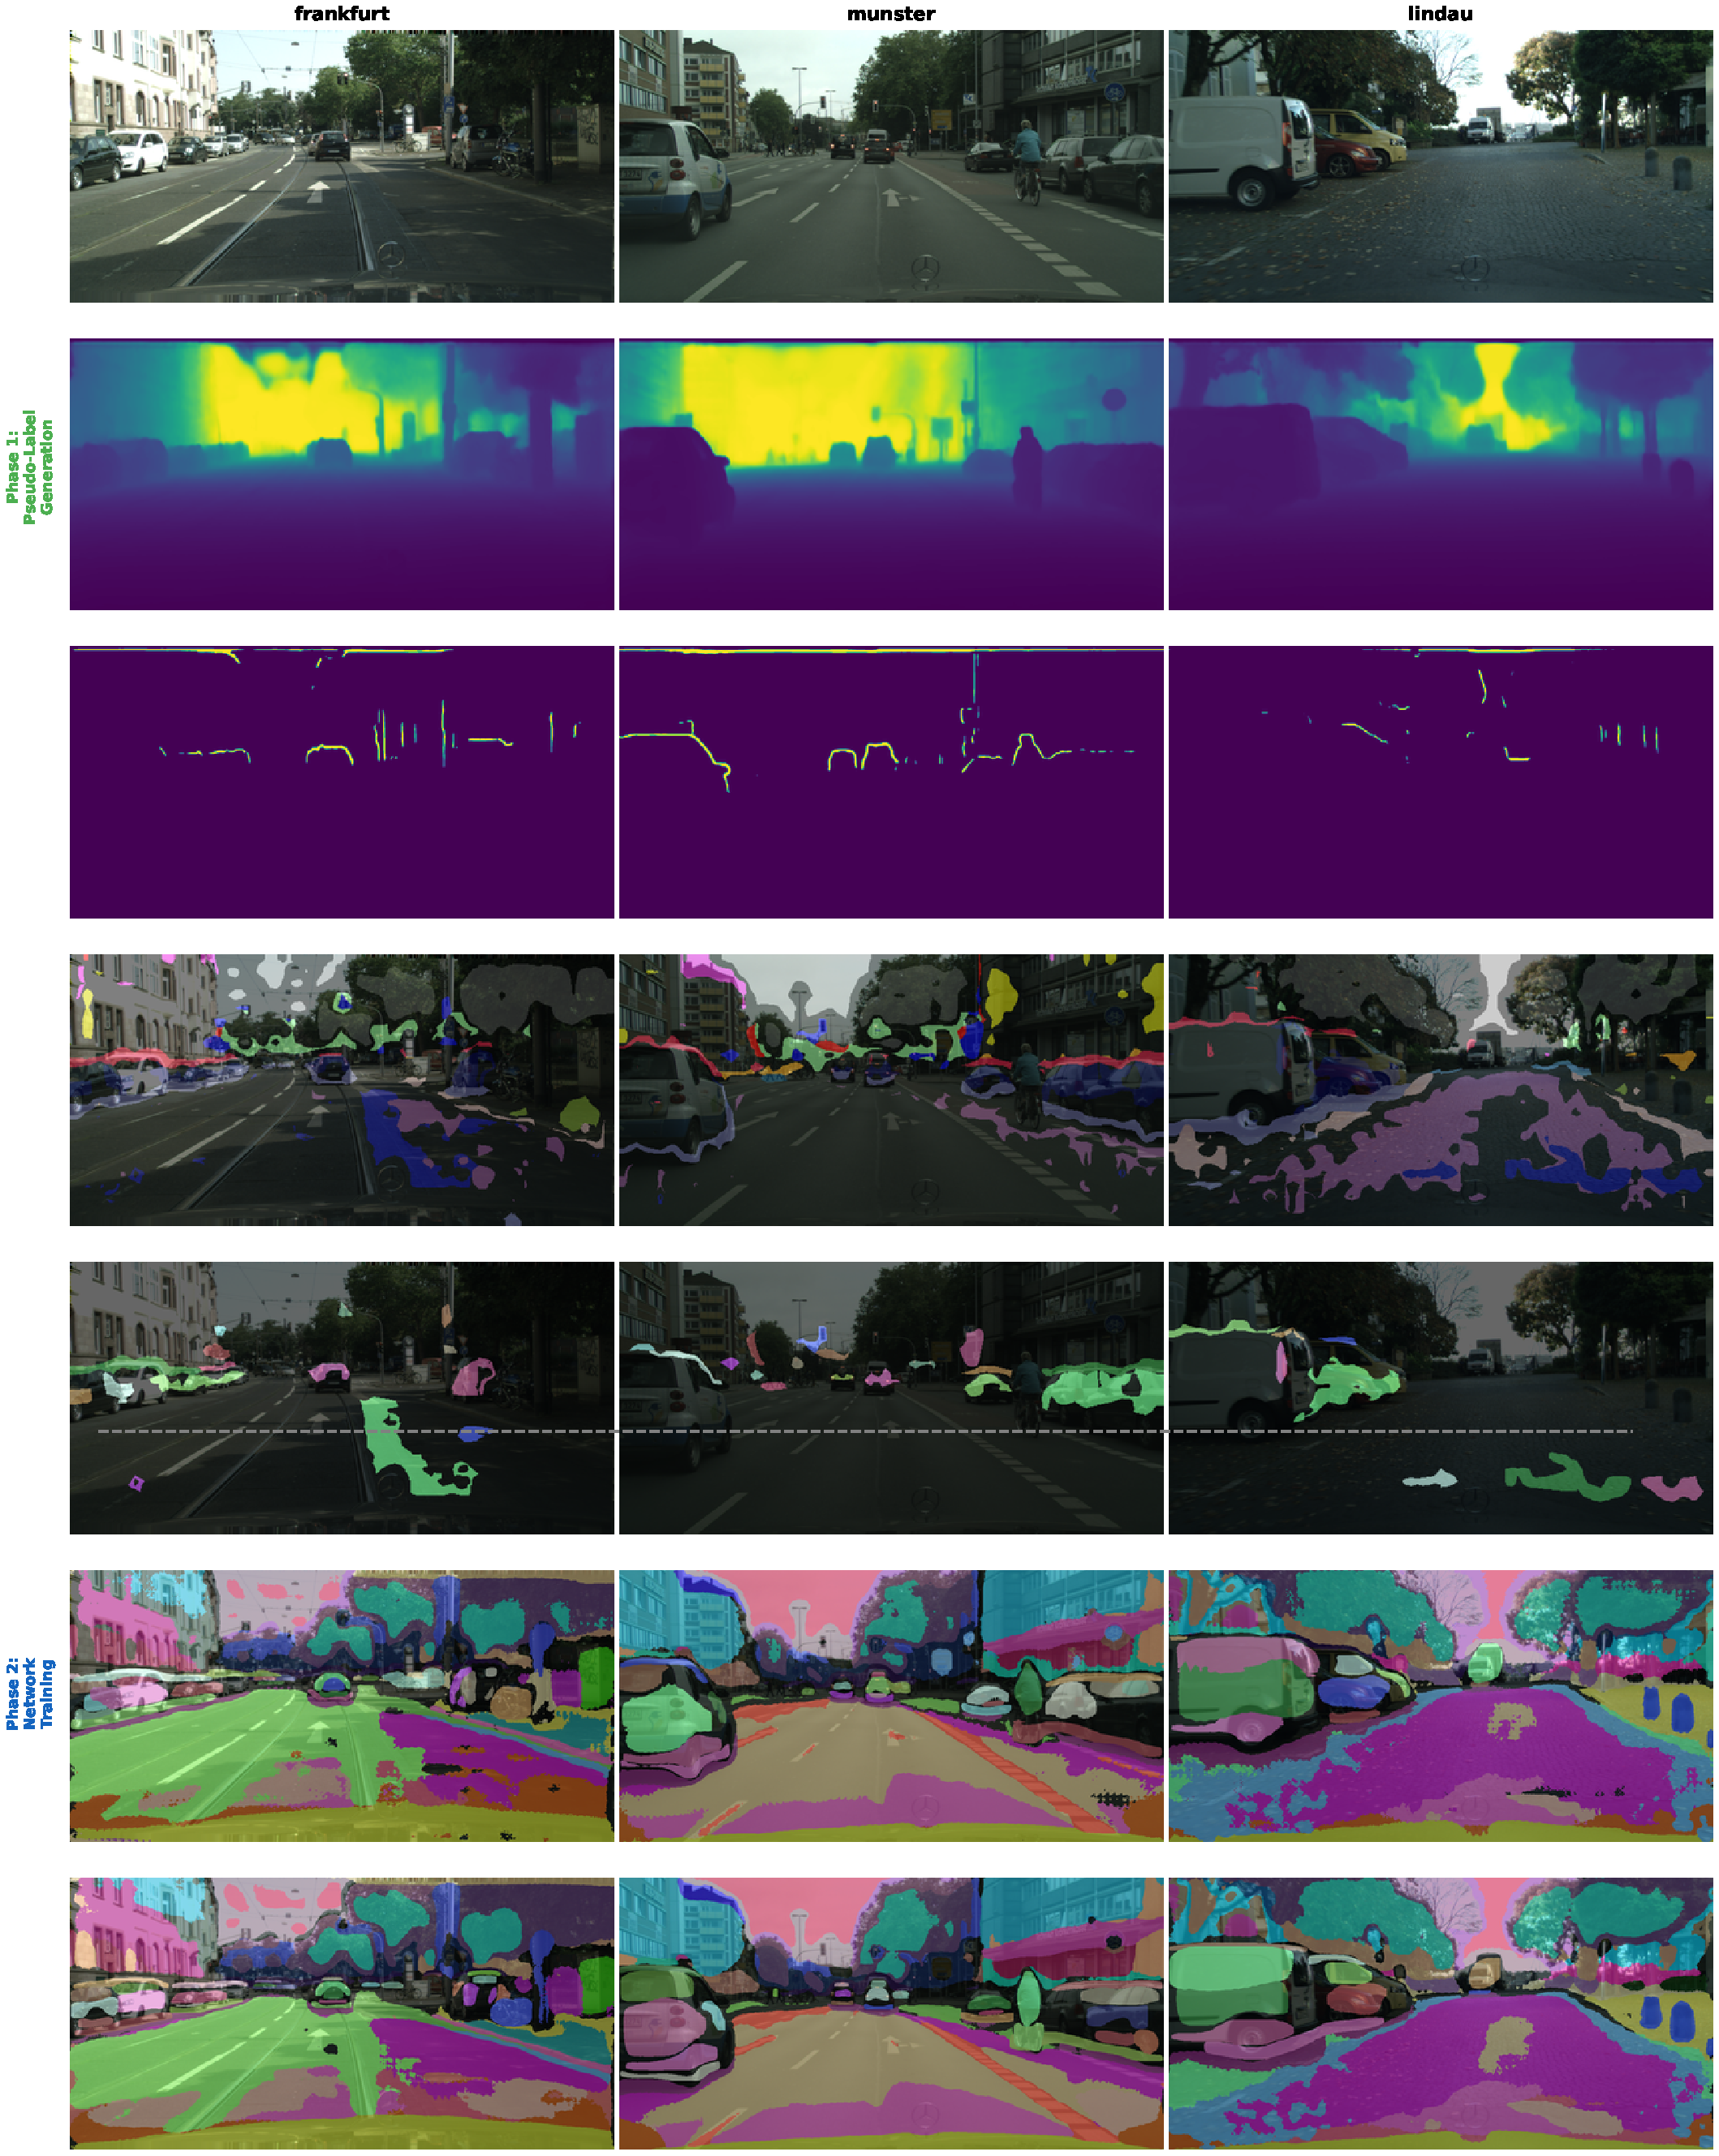
\includegraphics[width=\textwidth]{figures/fig5_qualitative.pdf}
\caption{\textbf{Full pipeline qualitative progression.} Rows: (a)~RGB input, (b)~monocular depth map, (c)~depth edges after Sobel thresholding (visualization uses SPIdepth, $\tau{=}0.20$; final method uses DAv3, $\tau{=}0.03$), (d)~semantic pseudo-labels ($k{=}80$), (e)~instance pseudo-labels from depth-guided splitting, (f)~Stage-2 panoptic prediction (PQ=27.87\%), (g)~Stage-3 panoptic prediction (PQ=32.76\%). Dashed line separates Phase~1 (pseudo-label generation) from Phase~2 (network training).}
\label{fig:qualitative}
\end{figure*}

%-------------------------------------------------------------------------
\section{Conclusion}

We have presented a fully unsupervised panoptic segmentation pipeline that composes frozen foundation models---a semantic feature clusterer (CAUSE-TR, $k{=}80$), a monocular depth estimator (DAv3), and a self-supervised backbone (DINOv3)---into a pseudo-label generation and training framework requiring no manual annotation. Our method achieves PQ=32.76\% on Cityscapes, surpassing CUPS (27.8\%) by +5.0 points, with strong gains in thing quality (\pqt: 34.1\% vs 17.7\%). Three findings carry broader implications: (1)~overclustering recovers seven collapsed classes in frozen CAUSE-TR features; (2)~monocular depth quality, not the splitting algorithm, is the binding constraint on instance pseudo-labels; and (3)~EMA self-training gains scale with teacher quality, from +1.25 PQ (ResNet-50) to +4.89 PQ (DINOv3).

\subsection*{Limitations}
The depth-guided splitting cannot separate co-planar objects (person PQ=4.2\%). Our frozen semantic pipeline cannot recover 7 non-standard CAUSE classes, creating a $-$3.1 \pqs ceiling versus CUPS. All results are from a single seed; the Stage-2 margin over CUPS (+0.07 PQ) is within noise. The self-training analysis rests on two backbone configurations; additional intermediate-capacity models would strengthen the characterization.

\FloatBarrier
\bibliography{references}

\end{document}
